\documentclass[tikz,border=10pt]{standalone}
\usepackage{tkz-euclide} % 用于方便地处理直角符号
\usetikzlibrary{calc,intersections}

\begin{document}
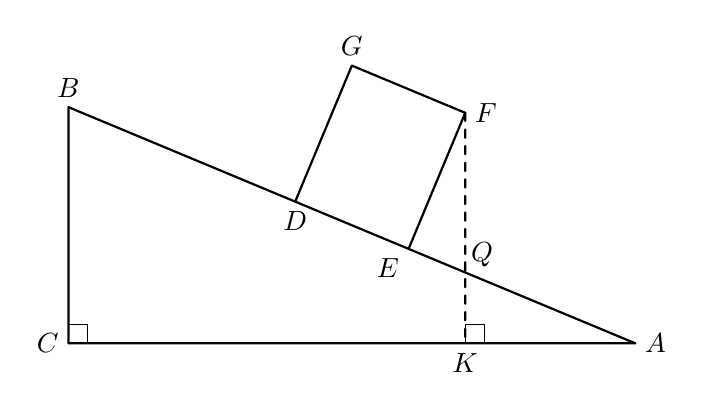
\begin{tikzpicture}[scale=1.2, line cap=round, line join=round]

    % --- 1. 定义核心顶点 (基于图像比例估算) ---
    \coordinate (C) at (0,0);
    \coordinate (A) at (6,0);
    \coordinate (B) at (0,2.5);

    % --- 2. 绘制大三角形 ABC ---
    \draw[thick] (A) -- (B) -- (C) -- cycle;

    % --- 3. 定义在斜边 AB 上的矩形 ---
    % 计算斜向角度
    \pgfmathsetmacro{\slopeangle}{atan2(2.5,-6)} % 计算 AB 的倾斜角
    
    % 在 AB 上选取 D 和 E 的位置 (使用线性插值)
    \coordinate (D) at ($(A)!0.6!(B)$);
    \coordinate (E) at ($(A)!0.4!(B)$);
    
    % 基于边 DE 向上构造矩形 DEFG
    % 矩形高度设为 1.2
    \coordinate (G) at ($(D) ! 1.2 ! 90:(E)$);
    \coordinate (F) at ($(E) ! 1.2 ! -90:(D)$);
    
    \draw[thick] (D) -- (G) -- (F) -- (E);

    % --- 4. 绘制投影辅助线 FK ---
    % K 是 F 在 AC 上的投影 (y 坐标与 C, A 相同)
    \coordinate (K) at (F |- C);
    \draw[dashed, thick] (F) -- (K);
    
    % 找到 FK 与 AB 的交点 Q
    \coordinate (Q) at (intersection of F--K and A--B);

    % --- 5. 绘制直角符号 ---
    \tkzMarkRightAngle[size=0.2](B,C,A)
    \tkzMarkRightAngle[size=0.2](F,K,A)

    % --- 6. 标注文本节点 ---
    \node[left] at (C) {$C$};
    \node[right] at (A) {$A$};
    \node[above] at (B) {$B$};
    \node[below] at (D) {$D$};
    \node[below left] at (E) {$E$};
    \node[right] at (F) {$F$};
    \node[above] at (G) {$G$};
    \node[below] at (K) {$K$};
    \node[above right=-2pt] at (Q) {$Q$};

\end{tikzpicture}
\end{document}